\documentclass[aspectratio=169]{beamer}

% because we need to claim weird things
\newtheorem{claim}{Claim}
\newtheorem{defn}{Definition}
%\newtheorem{lemma}{Lemma}
\newtheorem{thm}{Theorem}
\newtheorem{vita}{Vit\ae}
\newtheorem{qotd}{Quote of the Day}

\usepackage{algorithm}
\usepackage{algpseudocode}
\usepackage{listings}
\usepackage{color}
\usepackage{graphics}
\usepackage{ulem}
\bibliographystyle{unsrt}

% background image
\usebackgroundtemplate%
{%
    
\includegraphics[width=\paperwidth,height=\paperheight]{../artifacts/stemulus.pdf}%
}
\setbeamertemplate{caption}[numbered]
\lstset{%
	breaklines=true,
	captionpos=b,
	frame=single,
	keepspaces=true
}

% page numbers
\addtobeamertemplate{navigation symbols}{}{%
    \usebeamerfont{footline}%
    \usebeamercolor[fg]{footline}%
    \hspace{1em}%
    \insertframenumber/\inserttotalframenumber
}

% presentation header
\usetheme{Warsaw}
\title{Week 4: Introduction to JavaScript}
\author{Dylan Lane McDonald}
\institute{CNM STEMulus Center\\Web Development with PHP}
\date{\today}

\begin{document}
\lstset{language=HTML}
\begin{frame}
\titlepage
\end{frame}

\begin{frame}
\frametitle{Outline}
\tableofcontents
\end{frame}

\section{About JavaScript}
\subsection{History of JavaScript}
\begin{frame}
\frametitle{History of JavaScript}
JavaScript began its life at Netscape in 1995. Originally slated for Netscape 2.0, the language was originally called \textit{LiveScript} and subsequently renamed to \textit{JavaScript} shortly before Netscape 2.0's release. This begs the question: is JavaScript similar to Java?

\mbox{}\\
\pause
\textbf{ABSOLUTELY NOT!!!!}

\mbox{}\\
\pause
JavaScript's similarities to Java are purely superficial. The syntax is derived from a common ancestor, C, and both use C-like syntax. The similarities stop there.
\end{frame}

\subsection{Features of JavaScript}
\begin{frame}
\frametitle{Features of JavaScript}
JavaScript is an \textbf{interpreted} language run by a JavaScript engine, normally a component of the end user's web browser. Some of the key features of JavaScript are:
\begin{itemize}
	\item \textbf{Imperative}: Functions can be written to perform specific tasks
	\item \textbf{Object Oriented}: Objects can be modeled around what the system is
	\item \textbf{Dynamically Typed}: The variable type (e.g., String, Integer, \dots) are decided at run time 
\end{itemize}
JavaScript is enabled on most end user's web browsers and is used in creating responsive, dynamic, and fun sites.
\end{frame}

\section{JavaScript Syntax}
\subsection{Variables}
\begin{frame}
\frametitle{Variables}
\begin{defn}
A \textbf{variable} is a storage location and an associated symbolic name (an identifier) which contains some known or unknown quantity or information, a value. \cite{wiki-variable}
\end{defn}
\pause
A JavaScript variable is assigned like so:\\
\texttt{\textbf{var} answer = 42; // variable directly assigned\\
\textbf{var} question; // variable created with no value\\
\quad\quad$\vdots$\\
question = "What is the answer?"; // variable assigned later}
\end{frame}

\subsection{\texttt{if} Block}
\begin{frame}
\frametitle{\texttt{if} Block}
An \texttt{if} block is a decision point where JavaScript decides whether to perform one action or another. For instance:

\pause
\mbox{}\\
\texttt{if(answer == 42) \{\\
\quad console.log("We found the answer.");\\
\} else \{\\
\quad console.log("404 answer not found");\\
\}
}
\end{frame}

\subsection{Functions}
\begin{frame}
\frametitle{Functions}
\begin{defn}
A \textbf{function} is an executable unit that takes in zero or more inputs, performs a task, and returns zero or more outputs. Functions can be called multiple times with multiple inputs and are ideal for tasks that need to be performed many times.
\end{defn}

\pause
A good way to think of functions is to imagine yourself commanding a factory worker to go and perform a task for you. You tell the worker what to do and provide what he needs (input), he performs the task, and hands in the results (outputs).
\end{frame}

\begin{frame}
\frametitle{Functions}
\begin{figure}
\resizebox{60mm}{!}{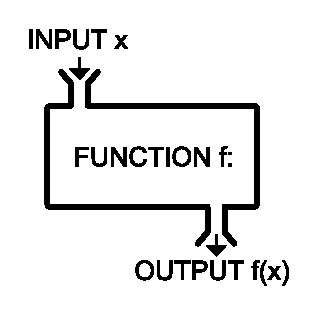
\includegraphics{../artifacts/function.pdf}}
\caption{Visual representation of a function}
\end{figure}
\end{frame}

\begin{frame}
\frametitle{Functions}
The syntax for functions are:\\
\mbox{}\\
// define function name \& inputs\\
\texttt{function addTwoNumbers(first, second) \{\\
\quad var sum = first + second; // perform task\\
\quad return(sum); // return the outputs\\
\}
}

\pause
\mbox{}\\
All functions start with the keyword \textbf{function}. Only functions that return an output end with a \textbf{return} statement.
\end{frame}


\begin{frame}
\frametitle{Works Cited}
\bibliography{javascript}
\end{frame}

\end{document}